\section{Voraussetzungen}

\subsection{Versuchsziel}

Ziel des Versuches $Z^0$-Resonanz ist das Nachzuvollziehen der Daten-Analyse des
L3-Experiments am LEP-Beschleuniger von 1989, aus der im Ergebnis die
Eigenschaften des damals neu entdeckten $Z^0$-Bosons, die Anzahl der
Quark-Farben und der elektroschwache Mischungswinkel hervorgehen.

\subsection{Physikalische Grundlagen}

Kollidieren ein Elektron und ein Positron, kann die inelastische Streuung durch
die elektromagnetische Wechselwirkung unter Austausch eines Photons vermittelt
werden, oder aber durch die schwache Wechselwirkung unter Austausch eines
sogenannten $Z^0$-Bosons. Bei hohen Schwerpunktsenergien $\sqrt{s}$ nahe der
$Z^0$-Masse $M_Z$ ist die elektromagnetische Wechselwirkung gegenüber der
schwachen jedoch stark unterdrückt.

Die $Z^0$-Resonanz bezeichnet den Kurven-Verlauf, der sich aus der
Berechnung des Wirkungsquerschnitts für den Zerfall
\begin{equation}
  e^{+} e^{-} \rightarrow Z^0 \rightarrow f \bar{f}
\end{equation}
ergibt und sein Maximum gerade bei einer Schwerpunktsenergie
$\sqrt{s}$, die der $Z^0$-Masse $M_Z$ entspricht, einnimmt. Die typische Form
der Breit-Wigner-Kurve resultiert hierbei aus dem entsprechenen Propagator,
wie im \cite[Gl. 2]{script} weiter ausgeführt wurde. Der Wirkungsquerschnitt für
ein Fermion $f$ mit der Zerfallsbreite des $Z^0$-Bosons $\Gamma_Z$ beträgt dann
\begin{equation}
  \label{eqn:sigmaf}
  \sigma_f = \sigma_0 \frac{s \Gamma_Z^2}{(s - M_Z^2)^2 + M_Z^2\Gamma_Z^2}
\end{equation}
mit dem Maximum $\sigma_0$ im Fall von $\sqrt{s} = M_Z$ bei
\begin{equation}
  \sigma_0 = \frac{12\pi}{M_Z^2}\frac{\Gamma_e\Gamma_f}{\Gamma_Z^2}
\end{equation}
. Hierbei ist $\Gamma_e$ die partielle Zerfallsbreite des Elektrons. Weiterhin gilt
für das Fermion mit Zerfallsbreite $\Gamma_f$ und elektrischer Ladung $Q_f$ nach
\cite[Gl. 6]{script} und Fermikonstante $G_F$ aus dem \cite{pdb}:
\begin{equation}
  \Gamma_f = \frac{G_F M_Z^3}{24 \sqrt{2}\pi}\left(1+[1-4|Q_f|\sin^2\Theta_W]^2\right)
\end{equation}

Bestimmt man nun experimentell Wirkungsquerschnitte der $Z_0$-Produktion in
Abhängigkeit von der Schwerpunktsenergie $\sqrt{s}$, so lassen sich mit einem
Fit an \eref{sigmaf} die Parameter $\sigma_0$, $M_Z$, $\Gamma_Z$ und mit
\begin{equation}
  \tau_Z = \frac{1}{\Gamma_Z}
\end{equation}
auch die Lebensdauer des $Z^0$-Bosons bestimmen.


\subsection{Versuchsaufbau}

\begin{figure}[htb]
 \centering
 \includegraphics[page=5,viewport=286 620 508 765,clip,%
  width=\columnwidth,keepaspectratio]{%
  ../docs/Z0ResFprakt}
 \caption{Aufbau das L3 Detektors}
 \label{fig:aufbau_detektor}
\end{figure}

Ausgangspunkt für diesen Versuch waren experimentell gemessene sowie auch
simulierte Daten. Es fand eine reine Datenauswertung statt.
Die Messdaten stammen aus dem L3-Experiment, welches am LEP-Beschleuniger betrieben wurde und dessen Aufbau in
\fref{aufbau_detektor} schematisch dargestellt ist.

Der Detektor ist aus mehreren Schichten aufgebaut,
wie es für moderne Teilchenbeschleuniger üblich ist. Alle Bereiche besitzen näherungsweise eine Zylinderform, wobei die Zylinderachse (z-Achse) in Strahlrichtung zeigt . Nahe am Strahlrohr befindet sich ein Spurdetektor, der in der Lage ist, die Bahnen geladener Teilchen zu verfolgen. In der Nähe des sogenannten Primär-Vertex’ (also des Wechselwirkungspunktes von Elektronen und Positronen) befindet sich auch ein Vertex-Detektor, um diesen Vertex-Punkt gut auflösen zu können.

Die darauf folgende, weiter außen liegende Schicht ist das elektromagnetische Kalorimeter, das vor allem die Energie von nicht stark wechselwirkenden Teilchen, also Photonen und Elektronen, messen soll. Die Kalorimeter bestehen aus einer Vielzahl einzelner Zellen, sodass Aussagen über den Ort, an dem ein Energiebetrag deponiert wurde, möglich sind.

Dahinter befindet sich das hadronische Kalorimeter, welches die Energiebeträge von hadronischen Teilchen messen soll. Es ist ebenfalls aus einzelnen Zellen zusammengesetzt.

Ganz außen schließlich folgen die Myonenkammern. Myonen durchdringen den inneren Teil des Detektors beinahe ungehindert, sodass sie die einzigen Teilchen sind, die dort noch registriert werden können.

% Man sollte noch erwähnen, dass sich auf den Zylinderflächen die Endkappen befinden. Das sind auch Kalorimeter, wobei die Reihenfolge die gleiche ist wie bei den Barrel-Kalorimetern (zuerst elektromagnetisches und dann hadronisches Kalorimeter).
Auf den Zylinderflächen befinden sich auch elektromagnetische und hadronische Kalorimeter, die Teilchenspuren nahe der z-Achse detektieren können.

In der Regel wird die genaue Impuls- und Energiemessung aus den Daten des Spurdetektors und der Kalorimeter gemeinsam rekonstruiert. Die zur Verfügung stehenden Daten enthalten nur die drei Impulskomponenten eines Teilchens sowie dessen Masse. Da die einzelnen Events in getrennten Blocks vorliegen, ist auch gegeben, wie viele Teilchen zu einem Event gehören. Die Energie eines Events lässt sich daraufhin leicht wieder rekonstruieren.
